\documentclass[11pt,a4paper]{article}
\usepackage[utf8]{inputenc}
\usepackage{graphicx}
\usepackage{geometry}
\usepackage{listings}
\usepackage{xcolor}
\usepackage{hyperref}
\usepackage{amsmath}
\usepackage{booktabs}

\geometry{margin=1in}

% Code listing style
\lstset{
    language=Python,
    basicstyle=\ttfamily\footnotesize,
    keywordstyle=\color{blue},
    stringstyle=\color{red},
    commentstyle=\color{gray},
    breaklines=true,
    frame=single,
    numbers=left,
    numberstyle=\tiny\color{gray}
}

\title{\textbf{Progress Report: LLMs as Evaluators for Code Metadata}\\
       \large Capstone Project}
\author{}
\date{\today}

\begin{document}

\maketitle

\section{Project Overview}

This project investigates the use of Large Language Models (LLMs) to evaluate and judge the quality of source code metadata, specifically focusing on code comments and documentation. The research employs Retrieval Augmented Generation (RAG) methods to enable LLMs to assess comment quality by leveraging structured program analysis and semantic context from real-world codebases.

The current phase has successfully implemented a complete pipeline that extracts structured metadata from a large-scale C codebase (libpng), creates navigable program maps, and deploys an LLM-powered agent capable of intelligent code navigation and metadata evaluation tasks.

\section{Implementation and Methodology}

\subsection{Static Code Analysis Pipeline}

The project implements a comprehensive static analysis system (\texttt{build\_map.py}) that processes the libpng repository (a mature, production-grade C library) to extract three critical types of program metadata:

\begin{enumerate}
    \item \textbf{Code Map}: Complete inventory of function definitions, including signatures, file locations, and line numbers, extracted using \texttt{ctags}
    \item \textbf{File Dependencies}: Include graph mapping header dependencies between files, extracted via \texttt{ripgrep}
    \item \textbf{Call Graph}: Function call relationships showing which functions are invoked by each source file, approximated using pattern matching
\end{enumerate}

The analysis pipeline leverages industry-standard tools:
\begin{itemize}
    \item \texttt{universal-ctags} for function definition extraction
    \item \texttt{ripgrep} for efficient pattern-based code analysis
    \item \texttt{graphviz} for generating scalable visualization outputs
\end{itemize}

\subsection{LLM Agent Architecture}

The agent system (\texttt{main.py}) integrates Google's Gemini 2.5 Flash model via the LlamaIndex framework. The agent is equipped with two specialized tools that enable retrieval-augmented code analysis:

\begin{itemize}
    \item \texttt{get\_code\_map\_info}: Queries structured metadata (code map, dependencies, or call graph) from the generated dataset
    \item \texttt{read\_source\_file}: Retrieves complete source code content from any file in the repository
\end{itemize}

The agent uses a ReAct (Reasoning + Acting) architecture, enabling it to:
\begin{itemize}
    \item Navigate the codebase systematically
    \item Combine structural metadata with source code context
    \item Provide grounded answers about code functionality and metadata quality
\end{itemize}

\section{Results and Outputs}

\subsection{Dataset Generation}

The static analysis pipeline successfully processed the entire libpng codebase, generating a comprehensive structured dataset:

\begin{table}[h]
\centering
\begin{tabular}{@{}lc@{}}
\toprule
\textbf{Metric} & \textbf{Count} \\
\midrule
Functions Indexed & 2,548 \\
Files with Dependencies & 81 \\
Files with Call Information & 88 \\
\bottomrule
\end{tabular}
\caption{Generated Dataset Statistics}
\end{table}

The dataset is stored in \texttt{code\_structure.json}, a structured JSON file containing all extracted metadata. This serves as the indexed input for LLM evaluation tasks.

\subsection{Sample Dataset Structure}

The generated \texttt{code\_structure.json} contains three main sections. Below is an example entry from the code map:

\begin{lstlisting}[caption={Sample Function Entry from code\_map}]
"png_get_cHRM": {
    "file": "pngget.c",
    "line": 526,
    "signature": "png_get_cHRM(png_const_structrp png_ptr, 
                 png_const_inforp info_ptr, 
                 double *whitex, double *whitey, 
                 double *redx, double *redy, 
                 double *greenx, double *greeny, 
                 double *bluex, double *bluey)"
}
\end{lstlisting}

\subsection{Visualization Outputs}

The pipeline generates scalable SVG visualizations that aid in understanding code structure. These visualizations are automatically converted to PDF format for inclusion in documentation and analysis.

\begin{figure}[h]
\centering
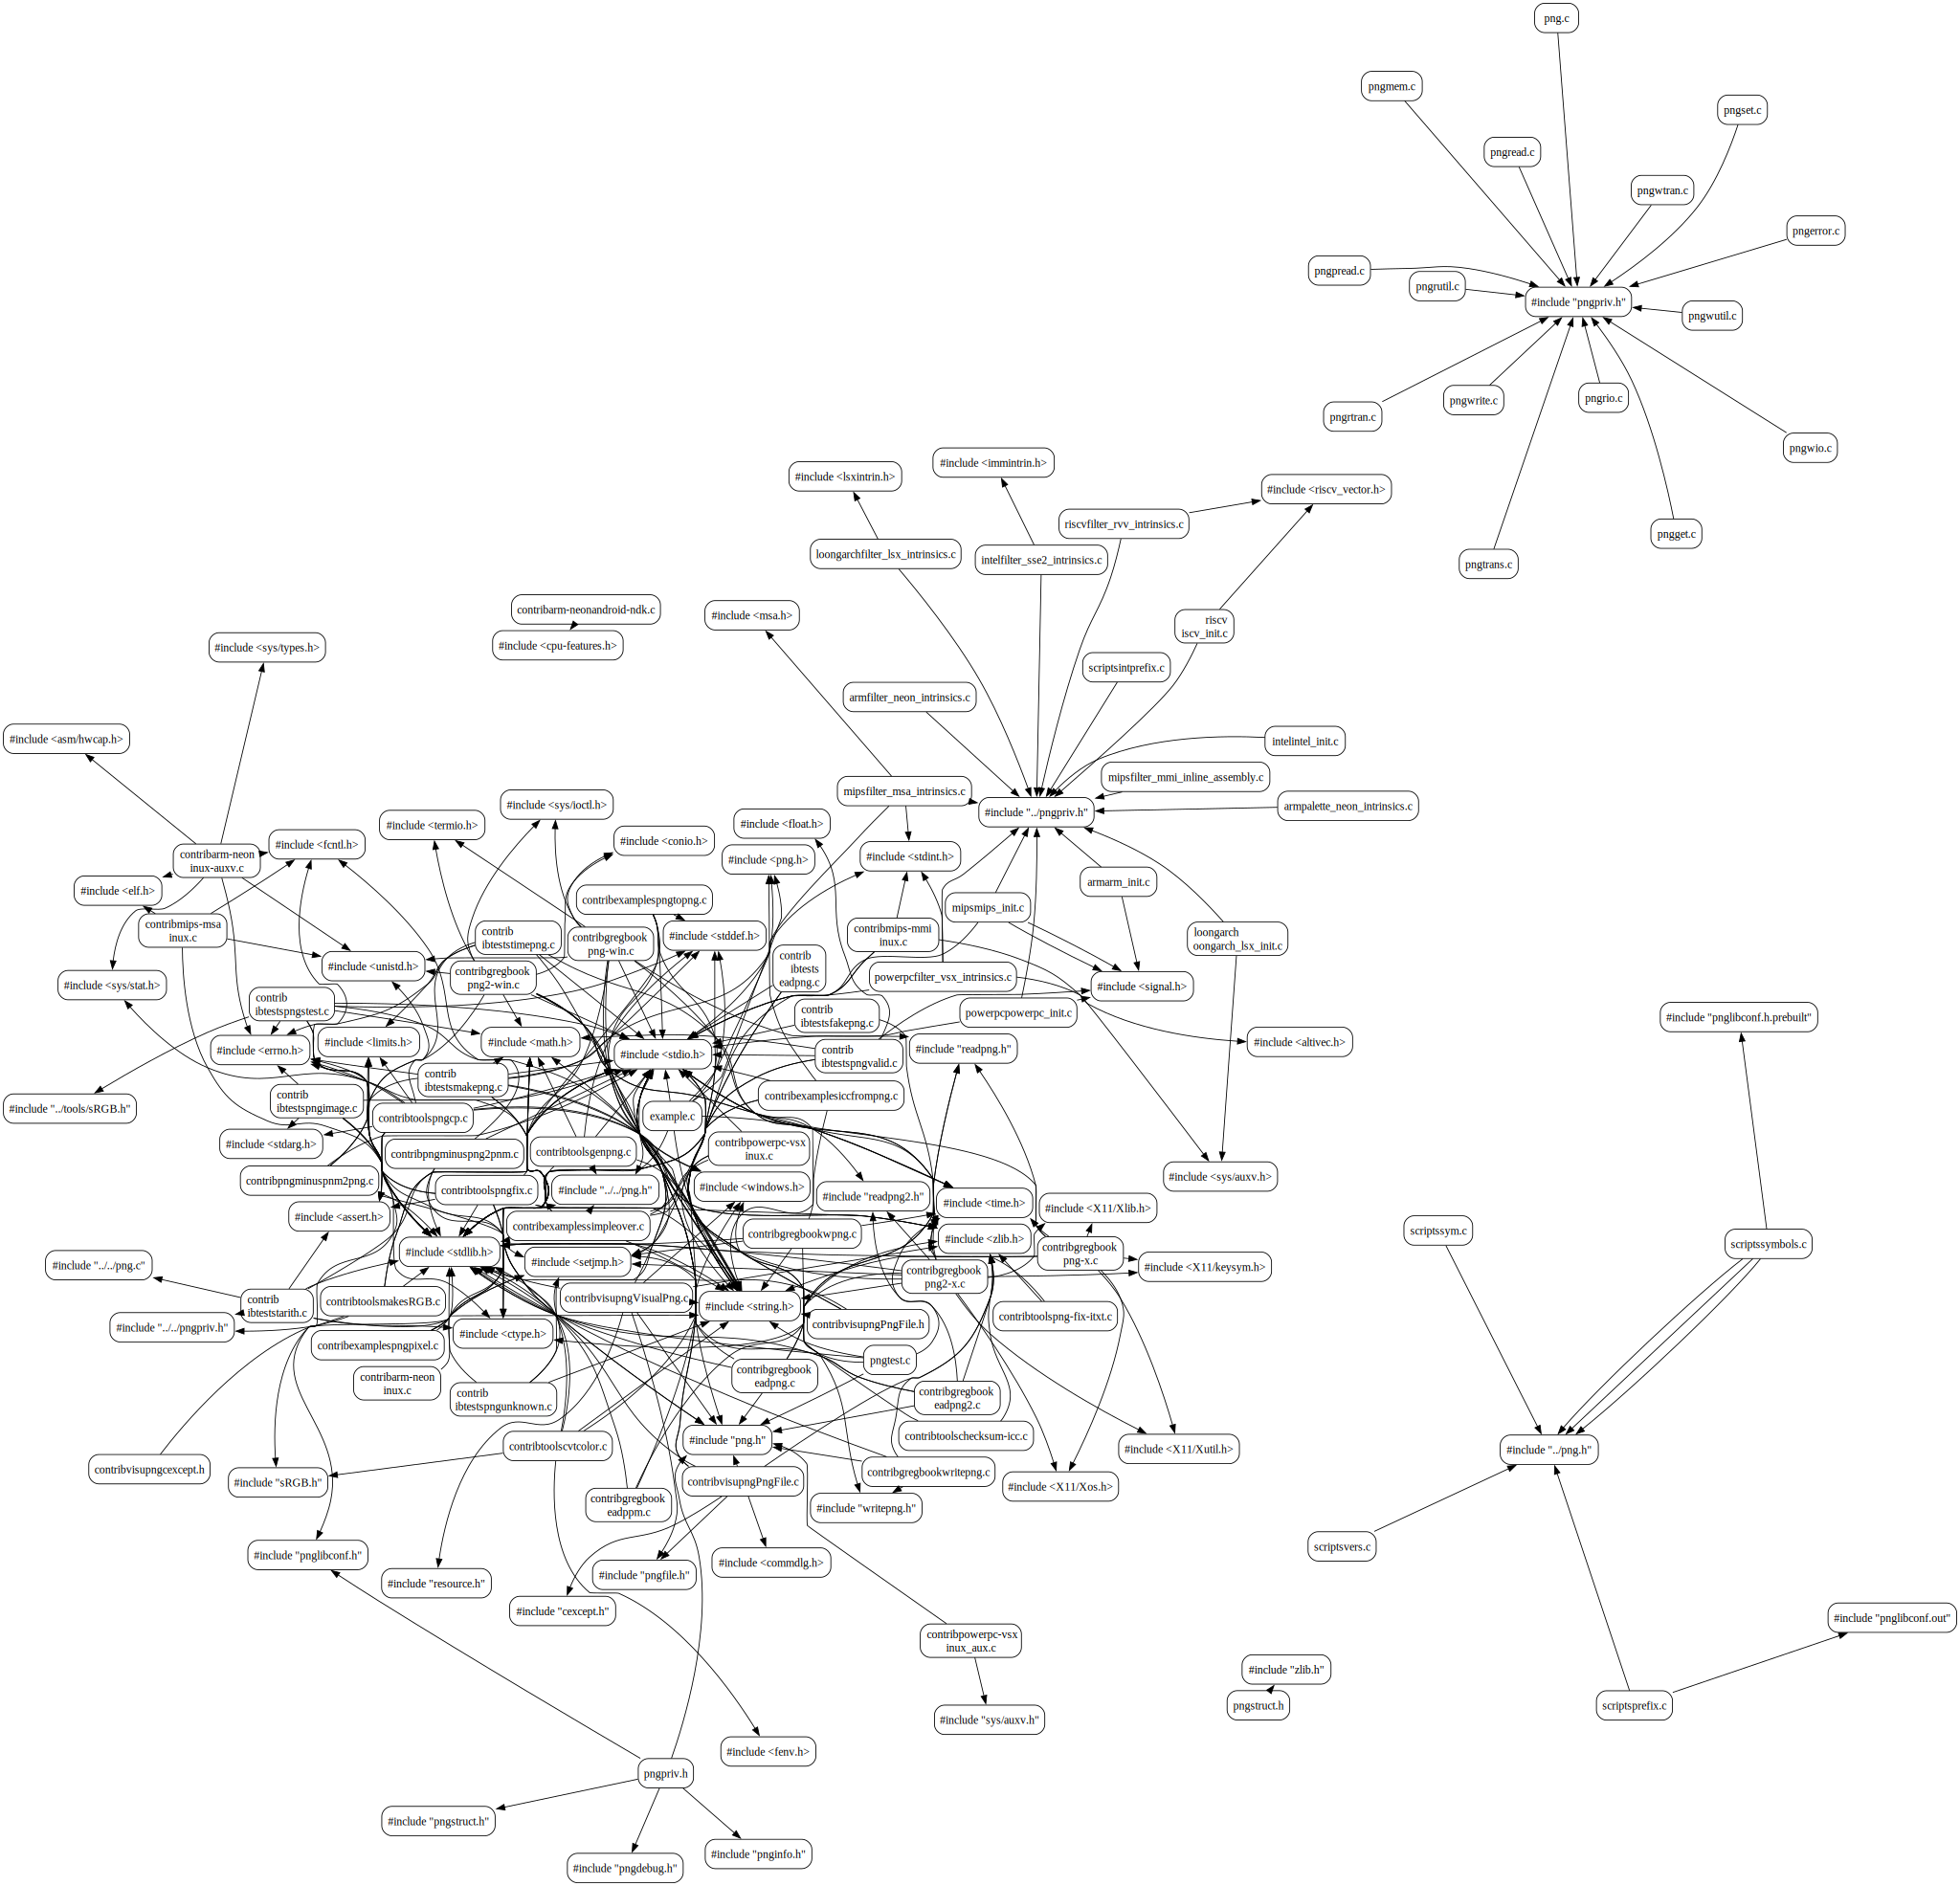
\includegraphics[width=0.9\textwidth]{file_dependencies.pdf}
\caption{File Dependency Graph: Complete dependency visualization showing header inclusion relationships between source files in the libpng codebase. This graph helps identify module coupling and dependency hierarchies.}
\label{fig:dependencies}
\end{figure}

\begin{figure}[h]
\centering

\includegraphics[width=0.9\textwidth]{call_map_pngread.pdf}
\caption{Call Map for \texttt{pngread.c}: Focused visualization showing all functions called by the \texttt{pngread.c} module. This targeted view demonstrates the complexity of function call relationships within a single critical file.}
\label{fig:pngread_calls}
\end{figure}

\begin{figure}[h]
\centering
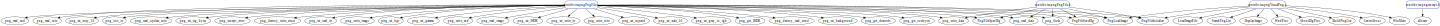
\includegraphics[width=0.9\textwidth]{call_map_visupng_module.pdf}
\caption{Call Map for \texttt{contrib/visupng} Module: Call graph visualization for the \texttt{contrib/visupng} directory, showing function call relationships within this module and connections to other parts of the codebase.}
\label{fig:visupng_calls}
\end{figure}

These visualizations provide human-readable representations of complex code relationships, enabling researchers to identify structural patterns and potential metadata evaluation targets. The focused views (Figures~\ref{fig:pngread_calls} and~\ref{fig:visupng_calls}) are particularly useful for understanding local call patterns, while the dependency graph (Figure~\ref{fig:dependencies}) reveals broader architectural relationships.

\subsection{Agent Performance Demonstration}

The LLM agent successfully demonstrates its capability to navigate the codebase and retrieve accurate information. In a test query asking for the function signature of \texttt{png\_get\_cHRM}, the agent:

\begin{enumerate}
    \item Used the \texttt{get\_code\_map\_info} tool to query structured metadata
    \item Navigated through multiple tool calls to locate the relevant information
    \item Retrieved the complete function signature with correct parameter types
\end{enumerate}

\textbf{Agent Response:}
\begin{verbatim}
png_get_cHRM(png_const_structrp png_ptr, png_const_inforp info_ptr, 
             double *whitex, double *whitey, double *redx, double *redy, 
             double *greenx, double *greeny, double *bluex, double *bluey)
\end{verbatim}

The agent's reasoning process is logged in \texttt{agent\_log\_*.txt} files, providing full transparency into the retrieval and reasoning steps.

\section{Achievements}

\subsection{Technical Accomplishments}

\begin{itemize}
    \item \textbf{Complete Pipeline Implementation}: Successfully built an end-to-end system from raw source code to structured metadata and LLM-powered analysis
    \item \textbf{Scalable Architecture}: The pipeline can process large codebases (2,500+ functions) efficiently using parallel tool execution
    \item \textbf{Structured Dataset Generation}: Created a reusable JSON schema that can be extended to multiple repositories for dataset building
    \item \textbf{Agent Tool Integration}: Demonstrated successful integration of program analysis tools with LLM agents using the LlamaIndex framework
\end{itemize}

\subsection{Research Contributions}

\begin{itemize}
    \item \textbf{Metadata Extraction Framework}: Established a systematic approach to extracting program structure, dependencies, and call relationships from C codebases
    \item \textbf{RAG Foundation}: Built the infrastructure for retrieval-augmented generation by creating structured, queryable code metadata
    \item \textbf{Evaluation Platform}: Created a working prototype that demonstrates LLM capability to evaluate code metadata quality using structural context
\end{itemize}

\subsection{Deliverables}

The following artifacts have been produced:

\begin{itemize}
    \item \texttt{build\_map.py}: Complete static analysis pipeline (354 lines)
    \item \texttt{main.py}: LLM agent system with tool integration (118 lines)
    \item \texttt{code\_structure.json}: Comprehensive structured dataset (15,000+ lines)
    \item Multiple SVG visualizations: Dependency and call graph representations
    \item Agent execution logs: Complete traces of LLM reasoning processes
\end{itemize}

\section{Next Steps}

The current implementation provides a solid foundation for the next phases:

\begin{enumerate}
    \item \textbf{Dataset Expansion}: Scale the pipeline to process multiple popular GitHub repositories to build a large-scale evaluation dataset
    \item \textbf{Comment Extraction}: Enhance the pipeline to extract and pair code comments with function definitions
    \item \textbf{Quality Metrics}: Implement rubric-based scoring for comment completeness, accuracy, and consistency
    \item \textbf{RAG Enhancement}: Integrate vector embeddings for semantic similarity search alongside structural retrieval
    \item \textbf{Evaluation Framework}: Develop systematic evaluation protocols for measuring LLM performance in metadata quality assessment
\end{enumerate}

\section{Conclusion}

This progress report demonstrates significant advancement toward the goal of using LLMs to evaluate code metadata quality. The implemented system successfully:

\begin{itemize}
    \item Extracts structured program metadata from a production codebase
    \item Creates navigable representations of code relationships
    \item Deploys an LLM agent capable of intelligent code navigation
    \item Provides a foundation for scalable metadata evaluation research
\end{itemize}

The infrastructure is ready for expansion to larger datasets and more sophisticated evaluation tasks, positioning the project well for the research track investigating scalability of LLM-based metadata analysis and generation.

\end{document}

